
\columnratio{0.55}
\begin{paracol}{2} 
\switchcolumn[0]*%%%%%%%
\section{Accessibility}
\switchcolumn
\section{无障碍访问}  
\switchcolumn[0]*%%%%%%%
Web accessibility (also known as a11y) refers to the practice of
creating websites that can be used by anyone --- be that a person with a
disability, a slow connection, outdated or broken hardware or simply
someone in an unfavorable environment. For example, adding subtitles to
a video would help both your deaf and hard-of-hearing users and your
users who are in a loud environment and can't hear their phone.
Similarly, making sure your text isn't too low contrast will help both
your low-vision users and your users who are trying to use their phone
in bright sunlight.
\switchcolumn
Web 无障碍访问 (也称为 a11y)
是指创建可供任何人使用的网站的做法------无论是身患某种障碍、通过慢速的网络连接访问、使用老旧或损坏的硬件,还是仅处于某种不方便的环境。例如,在视频中添加字幕可以帮助失聪、有听力障碍或身处嘈杂环境而听不到手机的用户。同样地,确保文字样式没有处于太低的对比度,可以对低视力用户和在明亮的强光下使用手机的用户都有所帮助。
\switchcolumn[0]*%%%%%%%
Ready to start but aren't sure where?
\switchcolumn
你是否已经准备开始却又无从下手?
\switchcolumn[0]*%%%%%%%
Checkout the
\href{https://www.w3.org/WAI/planning-and-managing/}{Planning and
managing web accessibility guide} provided by
\href{https://www.w3.org/}{World Wide Web Consortium (W3C)}
\switchcolumn
请先阅读由\href{https://www.w3.org/}{万维网联盟 (W3C)} 提供的
\href{https://www.w3.org/WAI/planning-and-managing/}{Web
无障碍访问的规划和管理}。
\end{paracol}



\columnratio{0.55}
\begin{paracol}{2} 
 
\switchcolumn[0]*%%%%%%%
\subsection{Skip link}
\switchcolumn
\subsection{跳过链接}
\switchcolumn[0]*%%%%%%%
You should add a link at the top of each page that goes directly to the
main content area so users can skip content that is repeated on multiple
Web pages.
\switchcolumn
你应该在每个页面的顶部添加一个直接指向主内容区域的链接,这样用户就可以跳过在多个网页上重复的内容。
\switchcolumn[0]*%%%%%%%
Typically this is done on the top of \texttt{App.vue} as it will be the
first focusable element on all your pages:
\switchcolumn
通常这个链接会放在 \texttt{App.vue}
的顶部,这样它就会是所有页面上的第一个可聚焦元素:
\switchcolumn[0]*%%%%%%%
\begin{codeHtml}
<ul class="skip-links">
  <li>
    <a href="#main" ref="skipLink" class="skip-link">Skip to main content</a>
  </li>
</ul>
\end{codeHtml}
\switchcolumn
\begin{codeHtml}
<ul class="skip-links">
  <li>
    <a href="#main" ref="skipLink" class="skip-link">Skip to main content</a>
  </li>
</ul>
\end{codeHtml}
\switchcolumn[0]*%%%%%%%
To hide the link unless it is focused, you can add the following style:
\switchcolumn
若想在非聚焦状态下隐藏该链接,可以添加以下样式:
\switchcolumn[0]*%%%%%%%
\begin{codeCss}
.skip-link {
  white-space: nowrap;
  margin: 1em auto;
  top: 0;
  position: fixed;
  left: 50%;
  margin-left: -72px;
  opacity: 0;
}
.skip-link:focus {
  opacity: 1;
  background-color: white;
  padding: 0.5em;
  border: 1px solid black;
}
\end{codeCss}
\switchcolumn
\begin{codeCss}
.skip-link {
  white-space: nowrap;
  margin: 1em auto;
  top: 0;
  position: fixed;
  left: 50%;
  margin-left: -72px;
  opacity: 0;
}
.skip-link:focus {
  opacity: 1;
  background-color: white;
  padding: 0.5em;
  border: 1px solid black;
}
\end{codeCss}
\switchcolumn[0]*%%%%%%%
Once a user changes route, bring focus back to the skip link. This can
be achieved by calling focus on the skip link's template ref (assuming
usage of \texttt{vue-router}):
\switchcolumn
一旦用户改变路由,请将焦点放回到这个``跳过''链接。通过如下方式聚焦``跳过''链接的模板引用
(假设使用了 \texttt{vue-router}) 即可实现:
\switchcolumn[0]*%%%%%%%
\begin{codeHtml}
<script setup>
import { ref, watch } from 'vue'
import { useRoute } from 'vue-router'
const route = useRoute()
const skipLink = ref()
watch(
  () => route.path,
  () => {
    skipLink.value.focus()
  }
)
</script>
\end{codeHtml}
\switchcolumn
\begin{codeHtml}
<script setup>
import { ref, watch } from 'vue'
import { useRoute } from 'vue-router'
const route = useRoute()
const skipLink = ref()
watch(
  () => route.path,
  () => {
    skipLink.value.focus()
  }
)
</script>
\end{codeHtml}
\switchcolumn[0]*%%%%%%%
\href{https://www.w3.org/WAI/WCAG21/Techniques/general/G1.html}{Read
documentation on skip link to main content}
\switchcolumn
\href{https://www.w3.org/WAI/WCAG21/Techniques/general/G1.html}{阅读关于跳过链接到主要内容的文档}
\end{paracol}



\columnratio{0.55}
\begin{paracol}{2} 
 
\switchcolumn[0]*%%%%%%%
\subsection{Content Structure}
\switchcolumn
\subsection{内容结构}
\switchcolumn[0]*%%%%%%%
One of the most important pieces of accessibility is making sure that
design can support accessible implementation. Design should consider not
only color contrast, font selection, text sizing, and language, but also
how the content is structured in the application.
\switchcolumn
确保设计可以支持易于访问的实现是无障碍访问最重要的部分之一。设计不仅要考虑颜色对比度、字体选择、文本大小和语言,还要考虑应用中的内容是如何组织的。
\switchcolumn[0]*%%%%%%%
\subsubsection{Headings}
\switchcolumn
\subsubsection{标题}
\switchcolumn[0]*%%%%%%%
Users can navigate an application through headings. Having descriptive
headings for every section of your application makes it easier for users
to predict the content of each section. When it comes to headings, there
are a couple of recommended accessibility practices:
\switchcolumn
用户可以通过标题在应用中进行导航。为应用的每个部分设置描述性标题,这可以让用户更容易地预测每个部分的内容。说到标题,有几个推荐的无障碍访问实践:
\switchcolumn[0]*%%%%%%%
\begin{itemize}
\item
  Nest headings in their ranking order:
  \texttt{\textless{}h1\textgreater{}} -
  \texttt{\textless{}h6\textgreater{}}
\item
  Don't skip headings within a section
\item
  Use actual heading tags instead of styling text to give the visual
  appearance of headings
\end{itemize}
\switchcolumn
\begin{itemize}
\item
  按级别顺序嵌套标题:\texttt{\textless{}h1\textgreater{}} -
  \texttt{\textless{}h6\textgreater{}}
\item
  不要在一个章节内跳跃标题的级别
\item
  使用实际的标题标记,而不是通过对文本设置样式以提供视觉上的标题
\end{itemize}
\switchcolumn[0]*%%%%%%%
\href{https://www.w3.org/TR/UNDERSTANDING-WCAG20/navigation-mechanisms-descriptive.html}{Read
more about headings}
\switchcolumn
\href{https://www.w3.org/TR/UNDERSTANDING-WCAG20/navigation-mechanisms-descriptive.html}{阅读更多有关标题的信息}
\switchcolumn[0]*%%%%%%%
\begin{codeHtml}
<main role="main" aria-labelledby="main-title">
  <h1 id="main-title">Main title</h1>
  <section aria-labelledby="section-title-1">
    <h2 id="section-title-1"> Section Title </h2>
    <h3>Section Subtitle</h3>
    <!-- 内容 -->
  </section>
  <section aria-labelledby="section-title-2">
    <h2 id="section-title-2"> Section Title </h2>
    <h3>Section Subtitle</h3>
    <!-- 内容 -->
    <h3>Section Subtitle</h3>
    <!-- 内容 -->
  </section>
</main>
\end{codeHtml}
\switchcolumn
\begin{codeHtml}
<main role="main" aria-labelledby="main-title">
  <h1 id="main-title">Main title</h1>
  <section aria-labelledby="section-title-1">
    <h2 id="section-title-1"> Section Title </h2>
    <h3>Section Subtitle</h3>
    <!-- 内容 -->
  </section>
  <section aria-labelledby="section-title-2">
    <h2 id="section-title-2"> Section Title </h2>
    <h3>Section Subtitle</h3>
    <!-- 内容 -->
    <h3>Section Subtitle</h3>
    <!-- 内容 -->
  </section>
</main>
\end{codeHtml}
\switchcolumn[0]*%%%%%%%
\subsubsection{Landmarks}
\switchcolumn
\subsubsection{Landmarks}
\switchcolumn[0]*%%%%%%%
\href{https://developer.mozilla.org/en-US/docs/Web/Accessibility/ARIA/Roles/landmark_role}{Landmarks}
provide programmatic access to sections within an application. Users who
rely on assistive technology can navigate to each section of the
application and skip over content. You can use
\href{https://developer.mozilla.org/en-US/docs/Web/Accessibility/ARIA/Roles}{ARIA
roles} to help you achieve this.
\switchcolumn
\href{https://developer.mozilla.org/en-US/docs/Web/Accessibility/ARIA/Roles/landmark_role}{Landmark}
会为应用中的章节提供访问规划。依赖辅助技术的用户可以跳过内容直接导航到应用的每个部分。你可以使用
\href{https://developer.mozilla.org/en-US/docs/Web/Accessibility/ARIA/Roles}{ARIA
role} 帮助你实现这个目标。
\end{paracol}


\begingroup
\LTleft=0pt \LTright=0pt
\begin{longtable}{@{\extracolsep{\fill}}|p{0.15\textwidth}|p{0.15\textwidth}|p{0.3\textwidth}|p{0.3\textwidth}|}
\hline
HTML&ARIA Role&地标的目的&Landmark Purpose\\\hline
header       & \verb|role="banner"|        & 主标题:页面的标题& Prime heading: title of the page\\\hline
nav          & \verb|role="navigation"|    & 适合用作文档或相关文档导航的链接集合 &Collection of links suitable for use when navigating the document or related documents  \\\hline
main         & \verb|role="main"|          & 文档的主体或中心内容  &The main or central content of the document. \\\hline
footer       & \verb|role="contentinfo"|   & 关于父级文档的信息:脚注/版权/隐私声明链接&Information about the parent document: footnotes/copyrights/links to privacy statement \\\hline
aside        & \verb|role="complementary"| & 用来支持主内容,同时其自身的内容是相对独立且有意义的 &Supports the main content, yet is separated and meaningful on its own content  \\\hline
*无对应元素*      & \verb|role="search"|        & 该章节包含整个应用的搜索功能 &This section contains the search functionality for the application\\hline
form         & \verb|role="form"|          & 表单相关元素的集合 &Collection of form-associated elements                                       \\\hline
section      & \verb|role="region"|        & 相关的且用户可能会导航至此的内容。必须为该元素提供 label&Content that is relevant and that users will likely want to navigate to. Label must be provided for this element \\\hline
\end{longtable}
\endgroup


\columnratio{0.55}
\begin{paracol}{2} 
 
\switchcolumn[0]*%%%%%%%
\begin{vueQuote}{TIP}
It is recommended to use landmark HTML elements with redundant landmark
role attributes in order to maximize compatibility with legacy
\href{https://caniuse.com/\#feat=html5semantic}{browsers that don't
support HTML5 semantic elements}.
\end{vueQuote} 
\switchcolumn
\begin{vueQuote}{TIP}
建议同时使用 landmark HTML 元素和 role
属性,以最大程度地兼容\href{https://caniuse.com/\#feat=html5semantic}{不支持
HTML5 语义元素的传统浏览器}。
\end{vueQuote} 
\switchcolumn[0]*%%%%%%%
\href{https://www.w3.org/TR/wai-aria-1.2/\#landmark_roles}{Read more
about landmarks}
\switchcolumn
\href{https://www.w3.org/TR/wai-aria-1.2/\#landmark_roles}{阅读更多有关标题的细节}
\switchcolumn[0]*%%%%%%%
\subsection{Semantic Forms}
\switchcolumn
\subsection{语义化表单}
\switchcolumn[0]*%%%%%%%
When creating a form, you can use the following elements:
\texttt{\textless{}form\textgreater{}},
\texttt{\textless{}label\textgreater{}},
\texttt{\textless{}input\textgreater{}},
\texttt{\textless{}textarea\textgreater{}}, and
\texttt{\textless{}button\textgreater{}}
\switchcolumn
当创建一个表单,你可能使用到以下几个元素:\texttt{\textless{}form\textgreater{}}、\texttt{\textless{}label\textgreater{}}、\texttt{\textless{}input\textgreater{}}、\texttt{\textless{}textarea\textgreater{}}
和 \texttt{\textless{}button\textgreater{}}。
\switchcolumn[0]*%%%%%%%
Labels are typically placed on top or to the left of the form fields:
\switchcolumn
标签通常放置在表格字段的顶部或左侧:
\switchcolumn[0]*%%%%%%%
\begin{codeHtml}
<form action="/dataCollectionLocation" method="post" autocomplete="on">
  <div v-for="item in formItems" :key="item.id" class="form-item">
    <label :for="item.id">{{ item.label }}: </label>
    <input
      :type="item.type"
      :id="item.id"
      :name="item.id"
      v-model="item.value"
    />
  </div>
  <button type="submit">Submit</button>
</form>
\end{codeHtml}
\switchcolumn
\begin{codeHtml}
<form action="/dataCollectionLocation" method="post" autocomplete="on">
  <div v-for="item in formItems" :key="item.id" class="form-item">
    <label :for="item.id">{{ item.label }}: </label>
    <input
      :type="item.type"
      :id="item.id"
      :name="item.id"
      v-model="item.value"
    />
  </div>
  <button type="submit">Submit</button>
</form>
\end{codeHtml}
\switchcolumn[0]*%%%%%%%
Notice how you can include
\texttt{autocomplete=\textquotesingle{}on\textquotesingle{}} on the form
element and it will apply to all inputs in your form. You can also set
different
\href{https://developer.mozilla.org/en-US/docs/Web/HTML/Attributes/autocomplete}{values
for autocomplete attribute} for each input.
\switchcolumn
请注意这里我们是如何在表单元素中引入
\texttt{autocomplete=\textquotesingle{}on\textquotesingle{}}
的,它将应用于表单中的所有 input 框。你也可以为每个 input 框都设置不同的
\href{https://developer.mozilla.org/en-US/docs/Web/HTML/Attributes/autocomplete}{autocomplete
attribute 的值}。
\switchcolumn[0]*%%%%%%%
\subsubsection{Labels}
\switchcolumn
\subsubsection{标签}
\switchcolumn[0]*%%%%%%%
Provide labels to describe the purpose of all form control; linking
\texttt{for} and \texttt{id}:
\switchcolumn
提供标签来描述所有表单控件的用途;使 \texttt{for} 和 \texttt{id}
链接起来:
\switchcolumn[0]*%%%%%%%
\begin{codeHtml}
<label for="name">Name</label>
<input type="text" name="name" id="name" v-model="name" />
\end{codeHtml}
\switchcolumn
\begin{codeHtml}
<label for="name">Name</label>
<input type="text" name="name" id="name" v-model="name" />
\end{codeHtml}
\switchcolumn[0]*%%%%%%%
If you inspect this element in your chrome developer tools and open the
Accessibility tab inside the Elements tab, you will see how the input
gets its name from the label:
\switchcolumn
如果你在 chrome 开发工具中检查这个元素,并打开 Elements 选项卡中的
Accessibility 选项卡,你将看到输入是如何从标签中获取其名称的:
\end{paracol}

\begin{center} 
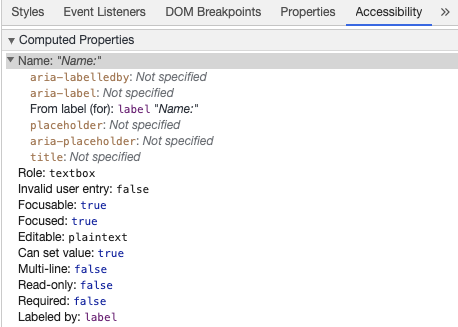
\includegraphics{./img/AccessibleLabelChromeDevTools.8d40e8fa.png} 
\end{center}
    

\columnratio{0.55}
\begin{paracol}{2} 
 
\switchcolumn[0]*%%%%%%%
\begin{vueQuoteWarn}{Warning:}
Though you might have seen labels wrapping the input fields like this:
\begin{codeHtml}
<label>
  Name:
  <input type="text" name="name" id="name" v-model="name" />
</label>
\end{codeHtml}
Explicitly setting the labels with a matching id is better supported by
assistive technology.
\end{vueQuoteWarn}
\switchcolumn
\begin{vueQuoteWarn}{警告:}
你可能还见过这样的包装 input 框的标签:
\begin{codeHtml}
<label>
  Name:
  <input type="text" name="name" id="name" v-model="name" />
</label>
\end{codeHtml}
但我们仍建议你显式地为 input 元素设置 id
相匹配的标签,以更好地实现无障碍访问。
\end{vueQuoteWarn}
\switchcolumn[0]*%%%%%%%
\paragraph{aria-label}
\switchcolumn
\paragraph{aria-label}
\switchcolumn[0]*%%%%%%%
You can also give the input an accessible name with
\href{https://developer.mozilla.org/en-US/docs/Web/Accessibility/ARIA/Attributes/aria-label}{\texttt{aria-label}}.
\switchcolumn
你也可以为 input 框配置一个带有
\href{https://developer.mozilla.org/en-US/docs/Web/Accessibility/ARIA/Attributes/aria-label}{\texttt{aria-label}}
的无障碍访问名。
\switchcolumn[0]*%%%%%%%
\begin{codeHtml}
<label for="name">Name</label>
<input
  type="text"
  name="name"
  id="name"
  v-model="name"
  :aria-label="nameLabel"
/>
\end{codeHtml}
\switchcolumn
\begin{codeHtml}
<label for="name">Name</label>
<input
  type="text"
  name="name"
  id="name"
  v-model="name"
  :aria-label="nameLabel"
/>
\end{codeHtml}
\switchcolumn[0]*%%%%%%%
Feel free to inspect this element in Chrome DevTools to see how the
accessible name has changed:
\switchcolumn
在 Chrome DevTools 中审查此元素,查看无障碍名称是如何更改的:
\end{paracol}

\begin{center} 
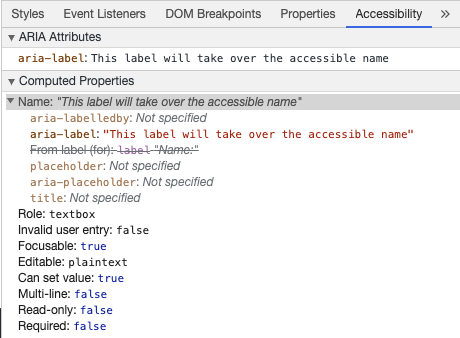
\includegraphics{./img/AccessibleARIAlabelDevTools.2b376a03.png} 
\end{center}
    
 
\columnratio{0.55}
\begin{paracol}{2} 
 
\end{paracol}


\columnratio{0.55}
\begin{paracol}{2} 

\end{paracol}



\columnratio{0.55}
\begin{paracol}{2} 

\end{paracol}



\columnratio{0.55}
\begin{paracol}{2} 

\end{paracol}



\columnratio{0.55}
\begin{paracol}{2} 

\end{paracol}


\columnratio{0.55}
\begin{paracol}{2} 

\end{paracol}



\columnratio{0.55}
\begin{paracol}{2} 

\end{paracol}



\columnratio{0.55}
\begin{paracol}{2} 

\end{paracol}


\columnratio{0.55}
\begin{paracol}{2} 

\end{paracol}



\columnratio{0.55}
\begin{paracol}{2} 

\end{paracol}


\columnratio{0.55}
\begin{paracol}{2} 

\end{paracol}



\columnratio{0.55}
\begin{paracol}{2} 

\end{paracol}


\columnratio{0.55}
\begin{paracol}{2} 

\end{paracol}



\columnratio{0.55}
\begin{paracol}{2} 

\end{paracol}



\columnratio{0.55}
\begin{paracol}{2} 

\end{paracol}



\columnratio{0.55}
\begin{paracol}{2} 

\end{paracol}


\columnratio{0.55}
\begin{paracol}{2} 

\end{paracol}



\columnratio{0.55}
\begin{paracol}{2} 

\end{paracol}



\columnratio{0.55}
\begin{paracol}{2} 

\end{paracol}


\columnratio{0.55}
\begin{paracol}{2} 

\end{paracol}



\columnratio{0.55}
\begin{paracol}{2} 

\end{paracol}